\section{Data models}

% Say something about how the graph is implemented and a reference to the book.
\subsection{DPF metamodeling}
\subsection{Entity model}

We will now present the entity model by showing en excerpt, hiding away the details. This will let us easier focus on the concepts and the flow, as the model itself is quite large and complex. See figure \ref{fig:EntityGraphExcerpt}

The entity graph shows a specific patient at a certain point or time in the clinical encounter. The patient comes to the emergency clinic. He has some symptoms which the clinician needs to uncover, by doing examinations and asking questions about the patients conditions. What the patient or caregiver tells is modelled as history, while quick examinations such as listening to the chest, looking at the skin, count the number of breaths per minute are modelled in the examination vertex. In some cases the clinician wants to test which require more time and resources, such as MRI scan, spirometry or blood tests, which are modelled as investigations.

Based on the the symptoms collected in history, examination and investigation, the clinician will set a diagnosis. The procedures for what to do with a patient with a given diagnosis is modelled under management. Hospitalization is to change the patients status to outpatient, or inpatient if he is admitted into the hospital. He might need some medication or be given advise for how he should deal with his condition the in every day life. Here the model can be expanded with routines found in other guidelines, we have identified surgery as an example. 
\begin{figure}[h!]
	\caption {An excerpt of the entity graph. Entity graph represents a patient at a certain point in the clinical encounter}
	\label{fig:EntityGraphExcerpt}
	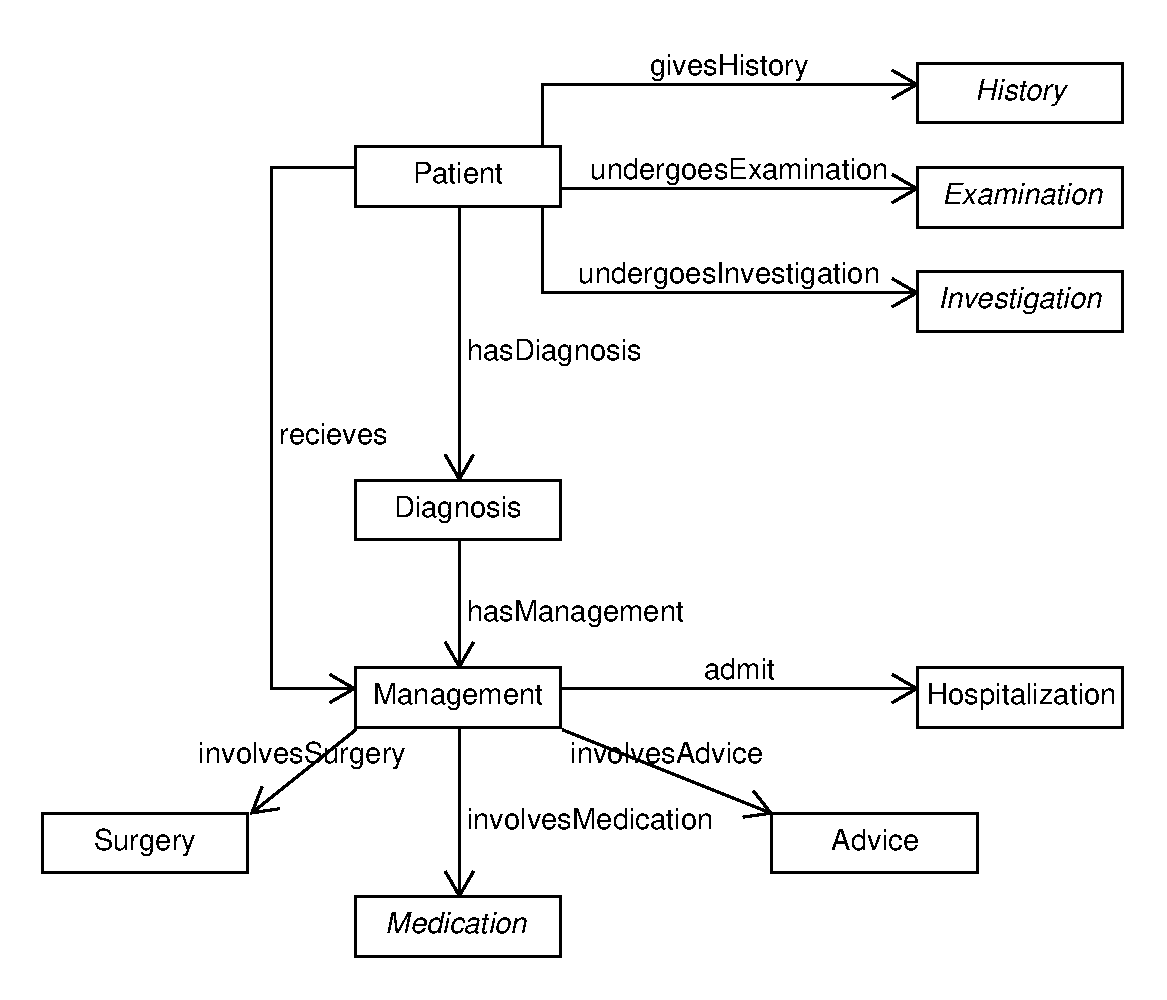
\includegraphics[scale=0.6]{EntityGraphExcerpt}
\end{figure}

In figure \ref{fig:EntityGraphPatientDiagnosis} we have expanded the Patient and Diagnosis vertices to reveal more details. PatientName and Gender, identifies the patient with a name and gender. These attributes are important when presenting a patient and his condition in a narrative or scenario. By using a name, it is easier for the reader to see that this is the same patient in different stages of the clinical encounter.

A diagnosis has a name. In the paediatric possible asthma guideline \cite{RepublicofKeny2016}, the diagnosis has a severity. A lot of medical conditions doesn't have a severity, or they are classified in another way. Here the model needs to be expanded to support other CPGs. 
\begin{figure}[h!]
	\caption {Showing the details of the Patient and Diagnosis vertices of the entity graph}
	\label{fig:EntityGraphPatientDiagnosis}
	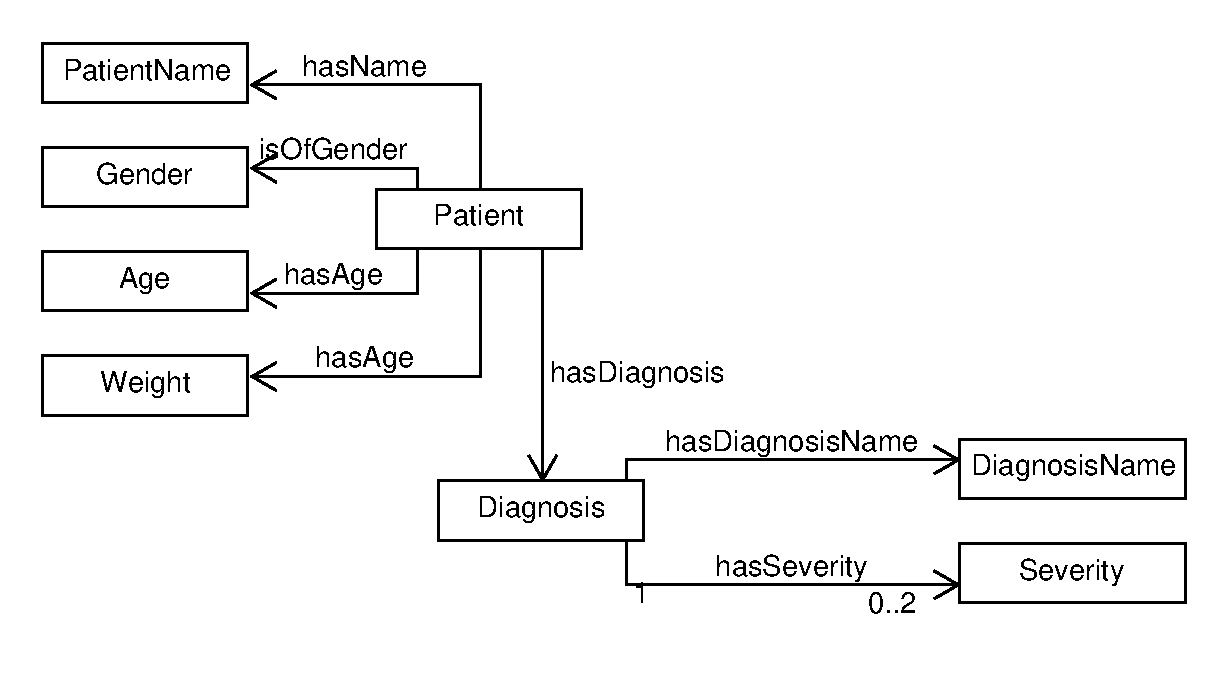
\includegraphics[scale=0.6]{EntityGraphPatientDiagnosis}
\end{figure}

\subsection{Workflow model}
\begin{figure}[h!]
	\caption {The workflow models is a model of the clinical encounter}
	\label{fig:WorkflowGraph}
	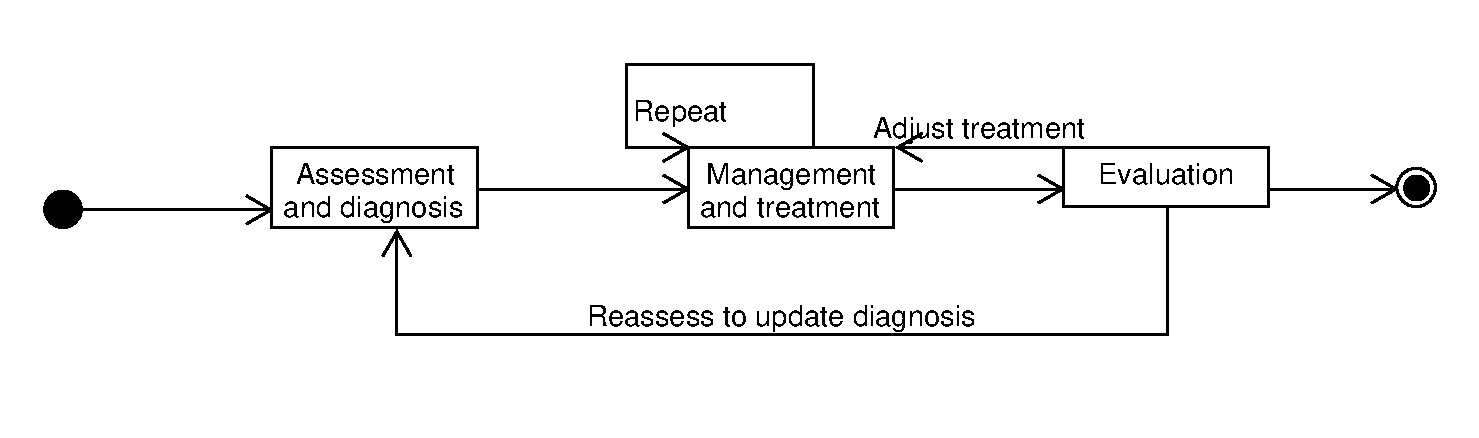
\includegraphics[scale=0.6]{WorkflowGraph}
\end{figure}


\subsection{Game model}